\section{Higgs zero mode III: cross terms with the nonzero modes}\label{rep:h-cross}

The gauge zero modes act on the non-zero modes of every charged field as constant connections, so the one-loop energy of Sec.~\ref{rep:h-matching} depends jointly on the Higgs radius $r$ and on the holonomies $(\bm x,\bm w)$.
Including all Standard Model fields, we find that these cross terms lower the critical top mass by $0.080$, $0.118$, and $0.160\GeV$ at $\Pone=0.9$, $1/2$, and $0.1$, with a model-internal error of $\pm0.008$, $\pm0.010$, and $\pm0.013\GeV$. %
We show that the antiperiodic fermions pin the hypercharge holonomy for every $r$, so that no instability of the soft $\bm w$ direction occurs; that the net sign comes from a hypercharge curvature that is nearly independent of $r$ while the tree-level stiffness of $\bm w$ grows with $r$; and that the one-loop logarithms of the Higgs--gauge-zero-mode terms close on the Higgs anomalous dimension (Sec.~\ref{sec:rb-r2c2}).
A blind calculation of the charged-component part, which carries all but $+0.005$ to $+0.007\GeV$ of the shift, gives $-0.081$, $-0.117$, and $-0.157\GeV$, against $-0.085$, $-0.124$, and $-0.167\GeV$ for the same part in our calculation; we keep the difference as an error (Sec.~\ref{rep:v-blind}). %

\subsection{Twisted sums and holonomy curvatures}
\label{sec:rb-twist}

We use the connection $D=\partial-i(A^aT_a+YB)$ with ${\rm tr}\,T_aT_b=\frac12\delta_{ab}$ and the constant modes $c=g_2\bm x$ and $u=g_Y\bm w$ in coordinates of unit period.
A field of charge $q$ in a constant background $\phi$ obeys $\psi(\bm x+\bm e_i)=e^{iq\phi_i}\psi(\bm x)$ after the background is gauged away, which is a twist of its boundary condition by $\bm\vartheta=q\bm\phi/2\pi$.
For one real degree of freedom of mass $m$ the finite-volume energy with twist $\bm\vartheta$ is the image sum of Eq.~(\ref{eq:rb-Etheta}), and its curvature at $\bm\vartheta=0$, the same in every direction by cubic symmetry, is
\begin{equation}
C(m)=\frac{\partial^2E_\vartheta}{\partial\vartheta_i^2}\Big|_0=\frac13m^2\sum_{\bm n\neq0}K_2(m|\bm n|)\times\begin{cases}1&\text{periodic},\\(-1)^{n_1+n_2+n_3}&\text{antiperiodic}.\end{cases}
\label{eq:rb-curv}
\end{equation}
Each real degree of freedom with statistics sign $s$ ($+1$ for bosons, $-1$ for fermions) and charge $q$ then contributes $s\,q^2C(m)/(4\pi^2)$ to the curvature of the one-loop energy in the holonomy $\phi$ [Fig.~\ref{fig:rb-diagrams}(e)].
For periodic fields the momentum mode $\bm k=0$ is a slow coordinate that belongs to the zero-mode dynamics, and we remove its contribution $2\pi^2/m$.
A direct mode sum, valid also for $m^2<0$, gives
\begin{equation}
C(m^2)=\tfrac23Z_1+2\pi^2\sum_{\bm k}{}'\Bigl[\frac{3m^2+2k^2}{3\omega^3}-\frac{2}{3k}\Bigr]+\frac{m^2}{6},
\label{eq:rb-curv-direct}
\end{equation}
where $\omega^2=k^2+m^2$ and $Z_1$ is $Z_P$ or $Z_A$ of Eq.~(\ref{eq:rb-tadpole}).
The summand is the direction-averaged second derivative of $\omega(\bm k-q\bm\phi)$, from which the massless value is subtracted; by Eq.~(\ref{eq:rb-noLog}) it falls as $k^{-5}$, so the curvature has no $\MSbar$ logarithm.
The last term is the difference between the cubic average on the lattice and the $d$-dimensional angular average of the continuum subtraction.
Hence $C=\frac23Z_1+m^2/6+O(m^4)$, and the two representations agree to $10^{-8}$--$10^{-10}$ for $m\ge0.6$; an independent Wolfram calculation with lattice shell sums agrees to $10^{-12}$. %

\paragraph{Curvatures at $r=0$.}
At $r=0$ all fields are massless and $C=\frac23Z_1$, so the curvature of a gauge factor is $\kappa=\sum s\,q^2Z_1/(6\pi^2)$ summed over its charged real degrees of freedom.
Counting the weights, for SU(3) the gluons contribute two polarizations times $2\cdot1^2+4\cdot(\frac12)^2$, a weight $6$, and the six quark flavors $4\times\frac12=2$ each; for SU(2) the $W$ bosons contribute $4$, the Higgs doublet $1$, and each of the twelve Weyl doublets $1$; for hypercharge the Higgs doublet contributes $1$ and the fermions $2\sum Y^2=20$, with $\sum Y^2=10/3$ per generation.
With the periodic bosons and antiperiodic fermions,
\begin{equation}
\kappa_3=\frac{6Z_P-12Z_A}{6\pi^2}=\frac{Z_P-2Z_A}{\pi^2},\qquad \kappa_2=\frac{5Z_P-12Z_A}{6\pi^2},\qquad
\kappa_Y=\frac{Z_P-20Z_A}{6\pi^2},
\label{eq:rb-kappas}
\end{equation}
where $Z_P=-8.913633$ and $Z_A=-2.519356$. %
Numerically $\kappa_3=-0.393$, $\kappa_2=-0.242$, and $\kappa_Y=+0.700$ (Sec.~\ref{rep:zeromodes}), and $\kappa_3/2$ reproduces the small-volume coefficient $-0.19631$ of Ref.~\cite{vanBaal:1988va}. %
With $\langle c^2\rangle=3.66$, $1.40$, and $0.82$ for the summed Gaussian widths of the SU(3), SU(2), and hypercharge zero modes, the first-order shift of the gauge ground state is %
\begin{equation}
\Delta Q=\tfrac12\kappa\langle c^2\rangle=-0.718-0.169+0.287=-0.601,
\label{eq:rb-DQ}
\end{equation}
as in Sec.~\ref{rep:zeromodes}. %
The hypercharge curvature is positive because the antiperiodic fermions pin the holonomy at its trivial value~\cite{vanBaal:1988va}: their weight exceeds that of the periodic Higgs doublet by $-20Z_A/|Z_P|=5.65$. %

\subsection{Cross terms at finite Higgs radius}
\label{sec:rb-hessian}

At $r>0$ the electroweak non-zero modes acquire the masses of Eq.~(\ref{eq:rb-masses}), and each real degree of freedom contributes with its own mass and charge.
In the body frame the vev component has $T^3=+\frac12$ and $Y=\frac12$ (the rotation $\bm N\to\bm e_3$ puts the vev in the upper component, so the unbroken generator is $T^3-Y$), and the background is the Cartan direction $g_2x^3T^3+g_YwY$.
We use a charged-component approximation (CCA):
\begin{itemize}
\item the transverse $W$ modes count four with $|T^3|=1$ and $m^2=a_W$;
\item each Coulomb mode carries the charge of its Goldstone boson with $m^2=a+b$, which equals $\omega_C^2$ of Eq.~(\ref{eq:rb-coulomb}) up to $O(ab/k^2)$;
\item the radial mode has $m^2=3\lambda r^2$;
\item the two top chiralities decouple, with $\tilde m_t$ as a vectorlike mass;
\item the light fermions are massless.
\end{itemize}
In the SU(2) direction transverse to the background the $W$ modes contribute two polarizations times $C(a_W)+c_W^2C(a_Z)+s_W^2C(0)$, where $c_W$ and $s_W$ are the cosine and sine of the weak mixing angle.
This gives a holonomy Hessian $H(r)$ in the components $(x^1,x^3,w)$.
The approximations of the CCA along the broken direction are removed in Sec.~\ref{sec:rb-r2c2} and in Sec.~\ref{sec:rb-xfinal} below.

\paragraph{Average over the conditional Gaussian.}
In the conditional Gaussian of Eq.~(\ref{eq:rb-condGauss}), $x^3=-\beta w+\delta x^3$ with $\langle(\delta x^3)^2\rangle=1/(2k)$ and $\langle(x^{1,2})^2\rangle=1/(2a)$ per direction.
Averaging $\frac12y^{\mathsf T}Hy$ over the SU(2) modes and summing over the three directions gives
\begin{equation}
E_X(r,\bm w)=E_X^x(r)+\tfrac12\Omega_X^2(r)|\bm w|^2,\qquad
E_X^x=\frac{3H_{11}}{2a}+\frac{3H_{33}}{4k},\qquad
\Omega_X^2=H_{ww}-2\beta H_{3w}+\beta^2H_{33},
\label{eq:rb-EX}
\end{equation}
where the first term comes from two charged components with $\langle(x^{1,2})^2\rangle=1/(2a)$ in three directions, the second from $\delta x^3$, and $\Omega_X^2$ from substituting $x^3=-\beta w$ in the $(x^3,w)$ block.
$E_X^x$ adds to the radial potential $U_1$ and $\Omega_X^2$ to the stiffness of the $\bm w$ channel of Eq.~(\ref{eq:rb-H2D}).

\paragraph{SU(3)--top term.}
The gluon zero modes commute with the Higgs field, so their curvature is exact at quadratic order,
\begin{equation}
\kappa_3(r)=\frac{6C_P(0)-2\bigl[5C_A(0)+C_A(\tilde m_t^2)\bigr]}{4\pi^2},
\label{eq:rb-kappa3}
\end{equation}
since only the top quark among the six flavors is massive at $\mub$.
The gluon zero modes add $\Delta U_3=\frac12[\kappa_3(r)-\kappa_3(0)]\langle c^2\rangle_3$ to the radial potential.
With $C_A(\tilde m_t^2)-C_A(0)=\tilde m_t^2/6+O(\tilde m_t^4)$ this is, at small $r$, a negative Higgs mass term,
\begin{equation}
\Delta U_3\simeq-\frac{\langle c^2\rangle_3\,\tilde m_t^2}{24\pi^2}=\tfrac12\delta m^2r^2,\qquad
\delta m^2=-\frac{\langle c^2\rangle_3\,y_t^2}{24\pi^2}=-0.0032/L^2
\label{eq:rb-dm2}
\end{equation}
at the fixed couplings ($-0.0028/L^2$ with $y_t(\mub)$). %
Physically, the top quark stiffens the gluon holonomy at small $r$ and decouples at large $r$.

\begin{table}[t]
\centering
\caption{Cross-term coefficients of the fixed-coupling estimate at $\lambda=-0.008$: the SU(2) part $E_X^x$ and its split into $W$, Higgs-doublet, top, and light-fermion loops, and the hypercharge curvature $\Omega_X^2$ (units $1/L$).
The dependence on $\lambda$ enters only through the radial and Goldstone masses and is below $10^{-3}$.} %
\label{tab:rb-hessian}
\begin{tabular}{ccccccc}
\toprule
$r$ & $E_X^x$ & $W$ & $H$ & $t$ & light & $\Omega_X^2$ \\
\midrule
$1$ & $-0.177$ & $-0.442$ & $-0.110$ & $+0.046$ & $+0.328$ & $0.136$ \\ %
$2$ & $-0.160$ & $-0.401$ & $-0.100$ & $+0.041$ & $+0.300$ & $0.135$ \\ %
$3$ & $-0.139$ & $-0.348$ & $-0.087$ & $+0.034$ & $+0.263$ & $0.131$ \\ %
$5$ & $-0.099$ & $-0.253$ & $-0.064$ & $+0.022$ & $+0.197$ & $0.118$ \\ %
\bottomrule
\end{tabular}
\end{table}

Table~\ref{tab:rb-hessian} gives the coefficients.
The hypercharge curvature stays positive for all $r\in[0,8]$, falling from $0.137$ to $0.105$; at $r=1$ the light fermions give $+0.142$, the top quark $+0.023$, the Higgs doublet $-0.029$, and the $W$ bosons through the photon content of $\beta$ only $-3\times10^{-5}$. %
It equals $+0.137$ for $r\le1.5$ and $+0.118$ at $r=5$. %
Keeping only the Higgs doublet gives $\Omega_X^2=-0.029$ for $r\le2$ and an inverted $\bm w$ direction for $r<0.776$; with all fields this apparent instability of the soft $\bm w$ direction is absent. %
The SU(2) curvature is negative, with the $W$ loop ($-0.60$) and the Higgs doublet ($-0.15$) outweighing the left-handed fermions ($+0.51$) in units of $c$. %
The masses decouple the periodic fields by only a few percent, since $C_P(m)$ changes by at most $5\%$, while the antiperiodic top decouples by about $26\%$ at $r=5$; the dependence on $r$ comes mainly from the zero-mode widths. %
Keeping only the Higgs fluctuations reproduces the earlier estimates of the matching study pointwise, which fixes the normalization. %

\paragraph{Light-fermion twist energy, exact in $s$.}
The light-fermion part of the hypercharge dependence is large, and we treat it exactly in $s=|\bm w|$.
For the s wave the twist energy of the massless antiperiodic fermions, averaged over the direction of $\bm w$, is
\begin{align}
V_L(r,s)&=-2\sum_\alpha n_\alpha\Bigl[\bar E_A\Bigl(\frac{|q_\alpha|s}{2\pi}\Bigr)-\bar E_A(0)\Bigr],\nonumber\\
\bar E_A(t)&=-\frac{1}{2\pi^2}\sum_{\bm n\neq0}\frac{(-1)^{|\bm n|^2}j_0(2\pi|\bm n|t)}{|\bm n|^4},
\label{eq:rb-VL}
\end{align}
where $n_\alpha$ counts the light Weyl fermions with charge $q_\alpha=g_YY-g_2\beta T^3$ along $\bm w$, $j_0$ is the spherical Bessel function from the angular average of $\cos(2\pi\bm n\cdot\bm\vartheta)$, and $(-1)^{|\bm n|^2}=(-1)^{n_1+n_2+n_3}$.
It rises monotonically and stays bounded over the whole $s$ box, so no instability appears at higher order.
The modes $\bm n=0$ and $\bm n=-1$ of a periodic field become degenerate at $|\vartheta|=\frac12$, which lies at $s\ge7.5$, while the two-dimensional wave function has probability below $10^{-8}$ at $s>6$; restricting to the fundamental domain therefore changes nothing. %
The $W$, Higgs, and top parts of $\Omega_X^2$ are kept to quadratic order.

\subsection{Variational treatment and the fixed-coupling estimate}
\label{sec:rb-var}

In a first estimate we add the cross terms at fixed couplings in two ways.
The first-order version adds $E_X^x+\Delta U_3$ to the radial potential and $\frac12\Omega_X^2s^2+V_L$ to the $\bm w$ channel.
The variational version adds the Gaussian average of the Hessian,
\begin{equation}
F=\frac{3H_{11}}{2a}+\frac34\,\frac{H_{33}e-2H_{3w}c+H_{ww}k}{D},
\label{eq:rb-F}
\end{equation}
to the Gaussian functional of Eq.~(\ref{eq:rb-moments}), minimizes again at every $r$, and rebuilds $C_0$, $B_x$, $\beta$, and $\Omega_{\rm eff}^2$ from the new parameters; this lowers $a$ by $3\%$.
For SU(3) we minimize $E(s)=\alpha/s+\beta_3s^2+\kappa_3(r)s/2$ over the summed width $s=\langle c^2\rangle_3$, with $\alpha$ and $\beta_3$ fixed by the Gaussian ground state ($E_0=8.603$, $s_0=3.66$); the curvature increases $s$ to $3.819$ and the SU(3) term by a factor $1.044$. %
The roots are found as in Sec.~\ref{sec:rb-siegert}; all 49 resonances converge inside their windows. %

\begin{table}[t]
\centering
\caption{Ratio of the static width with cross terms to the width of the two-dimensional model, in the fixed-coupling estimate (variational treatment), for all terms together and for each group of fields alone.} %
\label{tab:rb-ratios}
\begin{tabular}{ccccc}
\toprule
$\lambda$ & All & SU(3)--top & SU(2) & U(1)$_Y$ \\
\midrule
$-0.008$ & $1.629$ & $1.218$ & $0.645$ & $2.057$ \\ %
$-0.010$ & $1.566$ & $1.179$ & $0.682$ & $1.932$ \\ %
$-0.0143$ & $1.456$ & $1.124$ & $0.744$ & $1.720$ \\ %
\bottomrule
\end{tabular}
\end{table}

Table~\ref{tab:rb-ratios} shows that the hypercharge part dominates and increases the width, the SU(3)--top part also increases it, and the SU(2) part decreases it.
At $\lambda=0$ the cross terms shift the ground state by $+0.064$: $+0.238$ from hypercharge, which narrows $\langle s^2\rangle$ from $4.47$ to $2.98$, $-0.170$ from SU(2), and $-0.005$ from SU(3)--top. %
Converted with the hazard slopes, the fixed-coupling estimate moves the critical mass by $-0.093$, $-0.135$, and $-0.180\GeV$ at $\Pone=0.9$, $0.5$, and $0.1$. %
The groups alone give $-0.137$, $-0.196$, and $-0.258\GeV$ (U(1)$_Y$), $-0.035$, $-0.044$, and $-0.055\GeV$ (SU(3)--top), and $+0.080$, $+0.108$, and $+0.139\GeV$ (SU(2)); their sum differs from the joint result by at most $0.007\GeV$, and the first-order and variational versions differ by at most $0.003\GeV$. %
At $\Pone=1/2$ the three groups, taken one at a time, are about $-0.20$, $-0.04$, and $+0.11\GeV$, and their sum agrees with the joint result of this estimate to $0.004\GeV$. %

\subsection{Mechanism}
\label{sec:rb-xmech}

The sign of the total has a simple origin [Fig.~\ref{fig:rb-cross}(a)].
The hypercharge curvature $\Omega_X^2$ is nearly independent of $r$, while the tree-level stiffness of the $\bm w$ mode grows with $r$ ($\Omega_{\rm eff}\simeq g_Yr/2$ at small $r$).
The zero-point energy that the curvature adds to the $\bm w$ oscillator,
\begin{equation}
\delta E_w=\tfrac32\Bigl[\bigl(\Omega_{\rm eff}^2+\Omega_X^2\bigr)^{1/2}-\Omega_{\rm eff}\Bigr],
\label{eq:rb-dEw}
\end{equation}
is therefore larger in the well, $0.24$--$0.32/L$ at $r\approx1$--$1.5$, than at the barrier, $0.13$--$0.17/L$ at $r\approx3$--$5$. %
It lifts $\varepsilon$ toward the barrier top and increases $\Gamma$.
The top quark stiffens the gluon holonomy at small $r$ and decouples at large $r$, which acts like the negative Higgs mass term of Eq.~(\ref{eq:rb-dm2}) and also increases $\Gamma$.
The SU(2) curvature is negative and lowers the well more than the barrier, which decreases $\Gamma$.
The net effect is destabilizing: the cross terms lower the critical top mass.

\subsection{Node-direct cross terms with running couplings}
\label{sec:rb-xdirect}

The main calculation adds the cross terms at every node of the hazard with the node couplings $(g_2,g_Y,y_t,\lambda,g_3)$ and the NNLO mapping of Sec.~\ref{rep:h-smmap}.
At each node and for each $(m_t,\alpha_s)$ we
(i)~recompute the Hessian;
(ii)~minimize the Gaussian functional with $F$ again, starting from the optimum without cross terms (to $|\nabla|<10^{-8}$ for $r>0.05$);
(iii)~add the increments of $C_0$, $B_x$, and $\Omega_{\rm eff}^2$, computed with one discretization, to the baseline profile;
(iv)~add $\Omega_X^2$ and $V_L$ to the $\bm w$ channel and the SU(3)--top term with $E_0=12.98\,g_3^{2/3}$ and $s_0=3.66\,(g_3/0.5396)^{2/3}$; and
(v)~solve for the two-dimensional root. %
The summed SU(3) width scales as $g_3^{4/3}$ rather than $g_3^{2/3}$ (with $x=g^{-1/3}y$ the zero-mode Hamiltonian is $g^{2/3}$ times a $g$-independent one, so $\langle c^2\rangle=g^2\langle x^2\rangle\propto g^{4/3}$); with the node couplings the power used changes $s_0$ by less than $1\%$ where the hazard accumulates ($\tau\lesssim1.5$), which moves the SU(3)--top part by at most $4\times10^{-4}\GeV$, inside its width item in Table~\ref{tab:rb-xerr}. %
Without cross terms this code path reproduces the baseline roots to $1.3\times10^{-13}$ in $\varepsilon$ and $5\times10^{-12}$ relative in $\Gamma$. %
All 220 columns (ten masses at $\alpha_s=0.1180$ and five at each of $0.1171$ and $0.1189$, eleven nodes each) converge without flags in every run. %
The width ratio at the nodes is $1.53$ at $\tau=0$ and $1.57$ at $\tau=5$ for $m_t=172.6\GeV$, two to three percent below the fixed-coupling estimate because the node Yukawa coupling is smaller. %
The direct shifts are about $9\%$ smaller than the fixed-coupling conversion, which they replace. %

The numerics of the roots with cross terms were checked at $m_t=172.4$, $172.6$, $173.0$, and $173.4\GeV$ and at $\tau=0$, $2.5$, and $5$. %
A larger box, the base configuration of Table~\ref{tab:rb-widths}, a halved step, and $R_{\rm out}=14$ change $\Gamma$ by at most $6\times10^{-6}$ relative and $m_c$ by at most $3\times10^{-6}\GeV$; a zeroth-order outgoing condition changes $m_c$ by $-0.0003$, $-0.0002$, and $-0.0013\GeV$, so we take $0.001\GeV$ as the numerical error. %
Replacing the CCA average by the exact second-order curvature of the mixed mass bubbles,
\begin{equation}
q^2\sum_{\bm k}{}'\Bigl[\frac{1}{2\omega_1}+\frac{1}{2\omega_2}-\frac{2k_i^2}{\omega_1\omega_2(\omega_1+\omega_2)}\Bigr],
\label{eq:rb-mixedbubble}
\end{equation}
which for $\omega_1=\omega_2$ reduces to the CCA summand and differs from it by terms of order $k^{-5}$ otherwise, changes $m_c$ by at most $0.0005\GeV$. %

\subsection{Final result, decomposition, and errors}
\label{sec:rb-xfinal}

The CCA misses three one-loop terms of order $r^2c^2$ along the broken direction, derived in Sec.~\ref{sec:rb-r2c2}: the transverse vev mixing through the vertex $2(c\Phi_0)^\dagger V\delta\Phi$ of background-covariant Coulomb gauge, the Coulomb mismatch, and the exact top chiral loop.
With all three added at every node before the variational minimization, the critical masses are $172.502$, $172.960$, and $173.418\GeV$ at $\alpha_s(M_Z)=0.1180$, $0.080$, $0.118$, and $0.160\GeV$ below the two-dimensional model without cross terms. %
Relative to the CCA result ($172.498$, $172.954$, $173.412\GeV$) the gauge part shifts $m_c$ by $+0.021$, $+0.028$, and $+0.034\GeV$ and the top chiral loop by $-0.017$, $-0.022$, and $-0.027\GeV$, a net $+0.005$, $+0.006$, and $+0.007\GeV$; the cancellation reflects $\gamma_\phi^C\approx2\times10^{-4}$. %
The same shifts appear at $\alpha_s=0.1171$ and $0.1189$, where the final critical masses are $172.156$, $172.611$, $173.069\GeV$ and $172.849$, $173.308$, $173.768\GeV$. %

In the final model we also removed groups of terms at every node in two orders.
The SU(3)--top part is $-0.031$, $-0.039$, and $-0.046\GeV$ when removed first and $-0.032$, $-0.040$, and $-0.048\GeV$ when removed last, nearly independent of the order. %
The hypercharge and SU(2) parts together give $-0.048$, $-0.078$, and $-0.112\GeV$, close to the sum of their fixed-coupling values at $\Pone=1/2$, $-0.09\GeV$. %
The vev-mixing-plus-Coulomb and top-chiral groups give $+0.0214$, $+0.0275$, $+0.0336\GeV$ and $-0.0168$, $-0.0219$, $-0.0270\GeV$, and their sum reproduces the difference between the final and the CCA results to $2\times10^{-4}\GeV$. %
We quote the hypercharge and SU(2) parts together, with their separate sizes from the fixed-coupling estimate of Sec.~\ref{sec:rb-var}, because the root search did not converge in windows of $\pm0.02$ and $\pm0.10$ when either was removed alone in the final model; we did not establish whether the resonance left the windows or a box zero was selected. %

\begin{table}[t]
\centering
\caption{Model-internal error of the cross-term shift of $m_c$ (GeV) in the final model, combined in quadrature.} %
\label{tab:rb-xerr}
\begin{tabular}{p{0.52\textwidth}ccc}
\toprule
Item & $\Pone=0.9$ & $0.5$ & $0.1$ \\
\midrule
SU(2) and SU(3) widths, CCA, direction averaging, first order versus variational & $0.008$ & $0.010$ & $0.013$ \\ %
RG-closure residual & $0.0006$ & $0.0008$ & $0.0010$ \\ %
Custodial ratio for the $W$ Coulomb term & $0.0010$ & $0.0013$ & $0.0015$ \\ %
Neutral Coulomb fit, top numerics & $0.0003$ & $0.0003$ & $0.0004$ \\ %
Numerics & $0.001$ & $0.001$ & $0.001$ \\ %
\midrule
Total & $\pm0.008$ & $\pm0.010$ & $\pm0.013$ \\ %
\bottomrule
\end{tabular}
\end{table}

Table~\ref{tab:rb-xerr} lists the model-internal error.
Its first row collects the width of the SU(2) Gaussian (taken as $10\%$ of the SU(2) part), the charged-component approximation, the SU(3) width (Gaussian $3.66$ against virial $3.77$), direction averaging, and the difference between the first-order and variational treatments, scaled by the ratio $0.91$ of direct to fixed-coupling shifts. %
The RG-closure residual is at most $3\%$ of the gauge part and also covers the residual of a consistent scale variation; the custodial item is the $25\%$ uncertainty of the $W$-direction Coulomb term (Sec.~\ref{sec:rb-r2c2}). %
The conditions are those of the reduced model, together with the CCA for the electroweak Hessian, the quadratic treatment of the $W$, Higgs, and top parts of the hypercharge dependence, and the Gaussian width of the gluon zero modes.

The blind calculation of the CCA part (Sec.~\ref{rep:v-blind}), written from the model definitions for the Gaussian two-dimensional model with the earlier mapping and a twisted-sum approximation, gives $-0.081$, $-0.117$, and $-0.157\GeV$ against $-0.085$, $-0.124$, and $-0.167\GeV$ in the main calculation. %
Its groups, $-0.126$, $-0.179$, and $-0.237\GeV$ (U(1)$_Y$), $-0.031$, $-0.039$, and $-0.047\GeV$ (SU(3)--top), and $+0.082$, $+0.109$, and $+0.136\GeV$ (SU(2)), agree with the fixed-coupling estimate to within $0.022\GeV$, that is, to $9\%$ for the hypercharge and SU(2) parts and to $15\%$ for the smaller SU(3)--top part. %
We keep the difference, $\pm0.004$, $\pm0.007$, and $\pm0.010\GeV$, as a separate systematic error in the budget; it may overlap partly with the first-order-versus-variational item above, which errs on the conservative side. %
The vev mixing, the Coulomb mismatch, and the top chiral loop, which together move $m_c$ by $+0.005$ to $+0.007\GeV$, are checked within the main code by the RG closure, the exact top logarithm, and the additivity of the groups. %
Two-loop cross terms, such as the QCD correction to the top loop on the gluon holonomy, are not computed.

\begin{figure}[t]
\centering
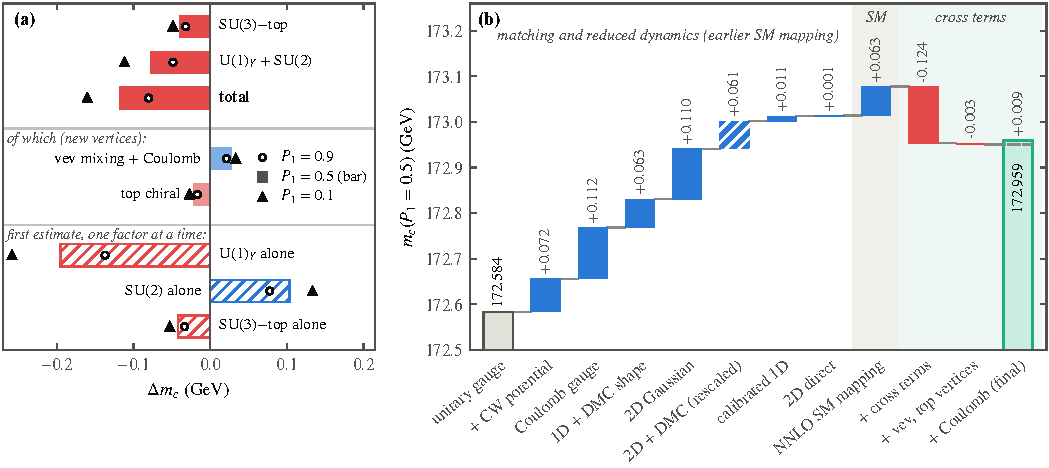
\includegraphics[width=\textwidth]{prd_cross_terms}
\caption{Zero-mode cross terms and the refinement of the critical mass.
(a)~Shift of $m_c$ by the one-loop cross terms (bars: $\Pone=0.5$; circles: $0.9$; triangles: $0.1$), split by gauge factor in the final model, with the new-vertex groups contained in the total, which is $-0.118\GeV$ at $\Pone=1/2$. %
Hatched: first estimate at fixed couplings, one gauge factor at a time (not additive).
(b)~$m_c(\Pone=1/2)$ along the model refinements of Table~\ref{tab:rb-convergence}, ending at $172.96\GeV$; the early steps add distinct physics rather than forming a convergence sequence, and the last two steps add the vev-mixing and top chiral vertices and then the Coulomb mismatch of the final model.} %
\label{fig:rb-cross}
\end{figure}
